\subsection{Riepilogo}
\subsubsection{Ore totali}
\subsubsubsection{Suddivisione lavoro}
La sequente tabella riporta il totale delle ore del progetto, sono presenti sia le ore rendicontate sia quelle di investimento.

\begin{table}[H]
	\begin{center}
	\rowcolors{2}{gray!25}{white}
	\renewcommand{\arraystretch}{1.25}
	\begin{tabular}{ m{0.20\textwidth}<{\centering}  m{0.06\textwidth}<{\centering} m{0.06\textwidth}<{\centering} m{0.06\textwidth}<{\centering}  m{0.06\textwidth}<{\centering}  m{0.06\textwidth}<{\centering}  m{0.06\textwidth}<{\centering}  m{0.20\textwidth}<{\centering}   }
		\rowcolor{darkblue}
		\textcolor{white}{\textbf{Componente}} &\textcolor{white}{\textbf{Re}}&\textcolor{white}{\textbf{Pt}}&\textcolor{white}{\textbf{An}}&\textcolor{white}{\textbf{Am}}&\textcolor{white}{\textbf{Pr}}&\textcolor{white}{\textbf{Ve}}&\textcolor{white}{\textbf{Ore complessive}}\\ 
		Edoardo Pavan & 20 & 15 & 15 & 16 & 40 & 24 & 130 \\	
		
		Francesco Protopapa & 20 & 20 & 25 & 15 & 35 & 20 & 135 \\
	
		Greta Cavedon & 20 & 15 & 25 & 17 & 32 & 25 & 135 \\
		
		Luciano Wu & 5 & 20 & 27 & 15 & 40 & 18 & 125 \\
		
		Matteo Basso & 10 & 15 & 20 & 25 & 30 & 20 & 120 \\
		
		Michele Gatto & 10 & 18 & 15 & 22 & 35 & 25 & 125 \\
		
		Pietro Villatora & 5 & 15 & 22 & 25 & 40 & 23 & 130 \\
		
		\textbf{Ore totali ruolo} & 90 & 118 & 149 & 135 & 252 & 155 & 900 \\
	
\end{tabular}
\caption{Distribuzione delle ore totali}
\end{center}
\end{table}

La tabella può essere rappresentata anche in forma visiva dal seguente grafico:
\begin{figure}[H]
\centering
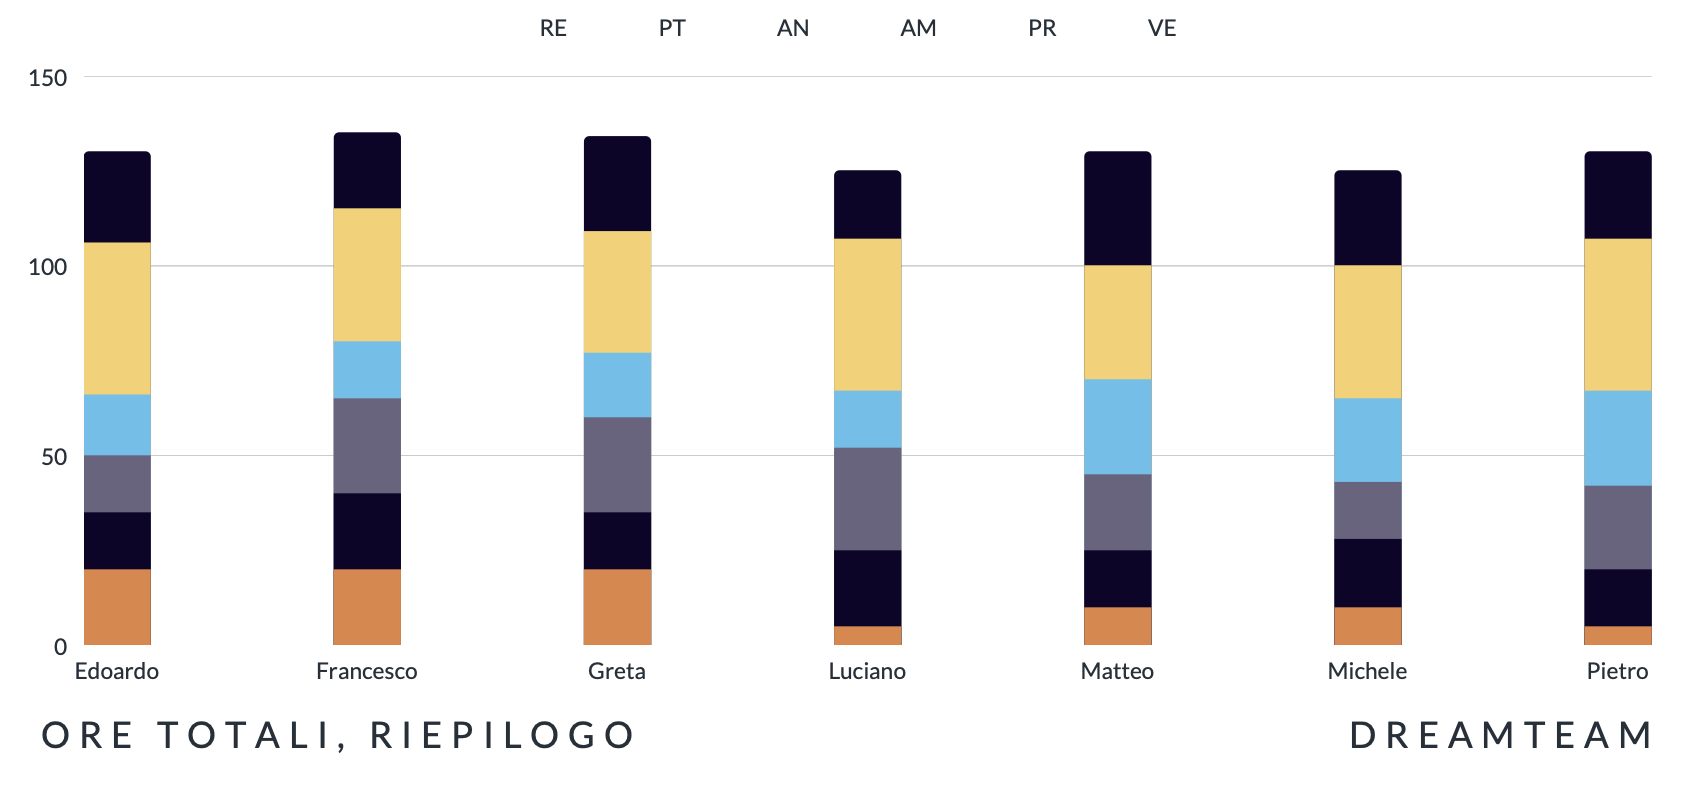
\includegraphics[scale=0.53]{Sezioni/SezioniPreventivo/grafici/Riepilogo_ore_totali.png}
\caption{Istogramma della ripartizione delle ore totali}
\end{figure}

\subsubsection{Prospetto economico}
La seguente tabella rappresenta le ore totali dedicate ad ogni ruolo e il costo in euro:

\begin{table}[H]
\begin{center}
\rowcolors{2}{gray!25}{white}
\renewcommand{\arraystretch}{1.5}
\begin{tabular}{ m{0.3\textwidth}<{\centering}  m{0.2\textwidth}<{\centering} m{0.2\textwidth}<{\centering}}
	\rowcolor{darkblue}
	\textcolor{white}{\textbf{Ruolo}}&\textcolor{white}{\textbf{Totale ore}}&\textcolor{white}{\textbf{Costo totale (\euro)}}\\ 

	Responsabile  & 90 & 2700 \\	
	
	Progettista & 118 & 2950 \\
	
	Analista & 149 & 3725 \\

	Amministratore & 135 & 2700 \\
	
	Programmatore & 252 & 3780 \\
	
	Verificatore & 155 & 2325 \\
	
	\textbf{Totale} & 900 & 18180 \\
	
\end{tabular}
\caption{Prospetto dei costi totali delle ore totali}
\end{center}
\end{table}

La tabella può essere rappresentata anche in forma visiva dal seguente aerogramma:
% \begin{figure}[H]
% \centering
% 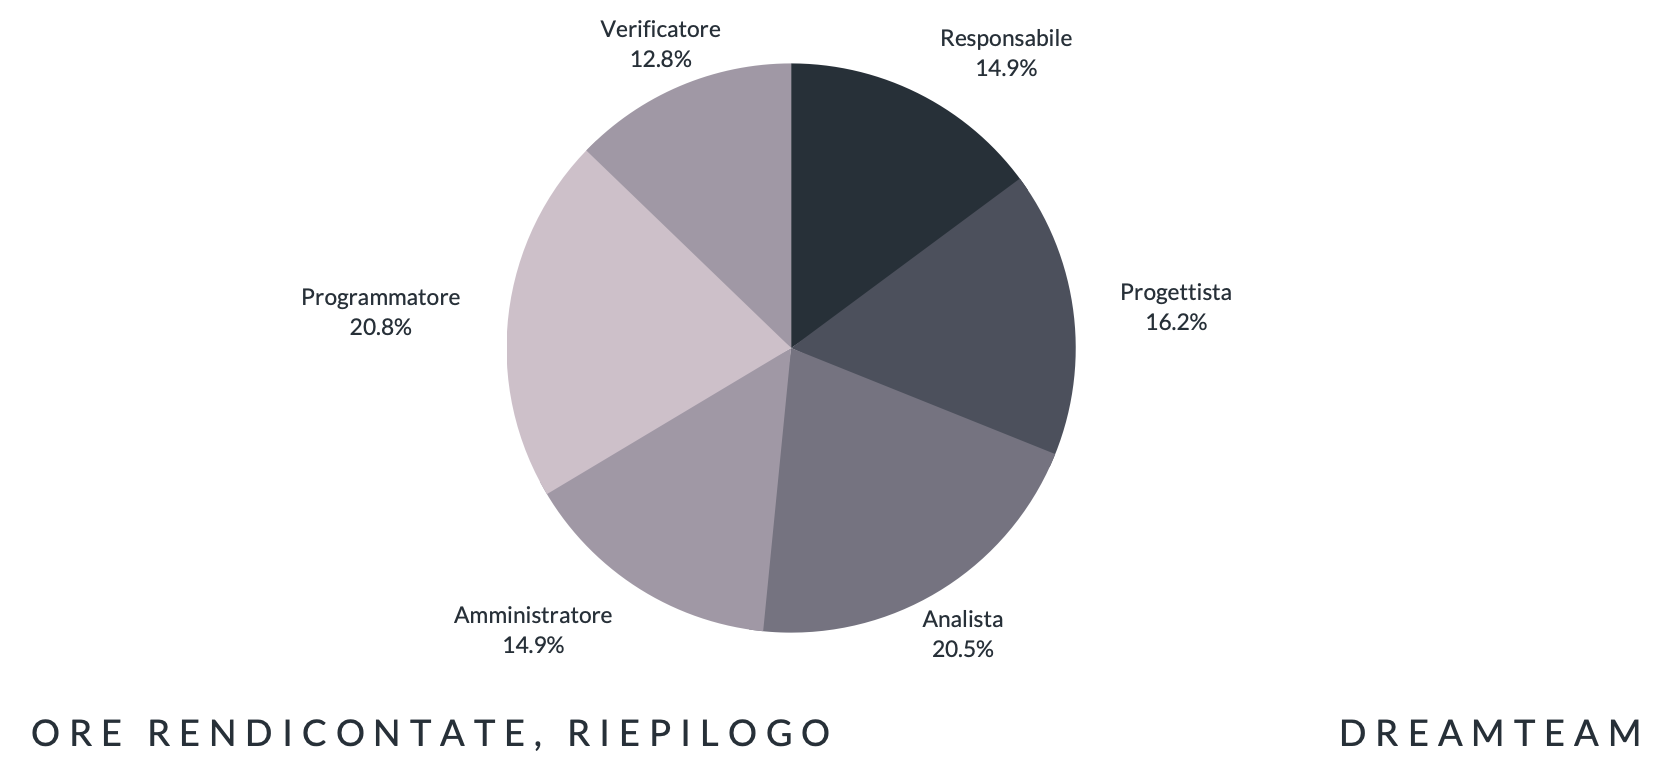
\includegraphics[scale=0.53]{Sezioni/SezioniPreventivo/grafici/Riepilogo_ore_totali_costi.png}
% \caption{Grafico a torta della ripartizione per ruolo delle ore totali}
% \end{figure}

\pagebreak

\subsubsection{Ore rendicontate}
\subsubsubsection{Suddivisione lavoro}
La seguente tabella riporta le ore rendicontate: 
\begin{table}[H]
\begin{center}
\rowcolors{2}{gray!25}{white}
\renewcommand{\arraystretch}{1.25}
\begin{tabular}{ m{0.20\textwidth}<{\centering}  m{0.06\textwidth}<{\centering} m{0.06\textwidth}<{\centering} m{0.06\textwidth}<{\centering}  m{0.06\textwidth}<{\centering}  m{0.06\textwidth}<{\centering}  m{0.06\textwidth}<{\centering}  m{0.20\textwidth}<{\centering}   }
	\rowcolor{darkblue}
	\textcolor{white}{\textbf{Componente}} &\textcolor{white}{\textbf{Re}}&\textcolor{white}{\textbf{Pt}}&\textcolor{white}{\textbf{An}}&\textcolor{white}{\textbf{Am}}&\textcolor{white}{\textbf{Pr}}&\textcolor{white}{\textbf{Ve}}&\textcolor{white}{\textbf{Ore complessive}}\\ 
	Edoardo Pavan & 10 & 14 & 10 & 11 & 15 & 20 & 80 \\	
	
	Francesco Protopapa & 10 & 10 & 20 & 5 & 35 & 20 & 100 \\

	Greta Cavedon & 15 & 10 & 20 & 4 & 26 & 25 & 100 \\
	1
	Luciano Wu & 5 & 20 & 20 & 5 & 38 & 12 & 100 \\
	
	Matteo Basso & 5 & 15 & 12 & 8 & 35 & 25 & 100 \\
	
	Michele Gatto & 8 & 16 & 5 & 12 & 35 & 24 & 100 \\
	
	Pietro Villatora & 5 & 15 & 10 & 12 & 38 & 20 & 100 \\
	
	\textbf{Ore totali ruolo} & 58 & 100 & 97 & 57 & 222 & 146 & 680 \\

\end{tabular}
\caption{Distribuzione delle ore rendicontate}
\end{center}
\end{table}

La tabella può essere rappresentata anche in forma visiva dal seguente grafico:
\begin{figure}[H]
\centering
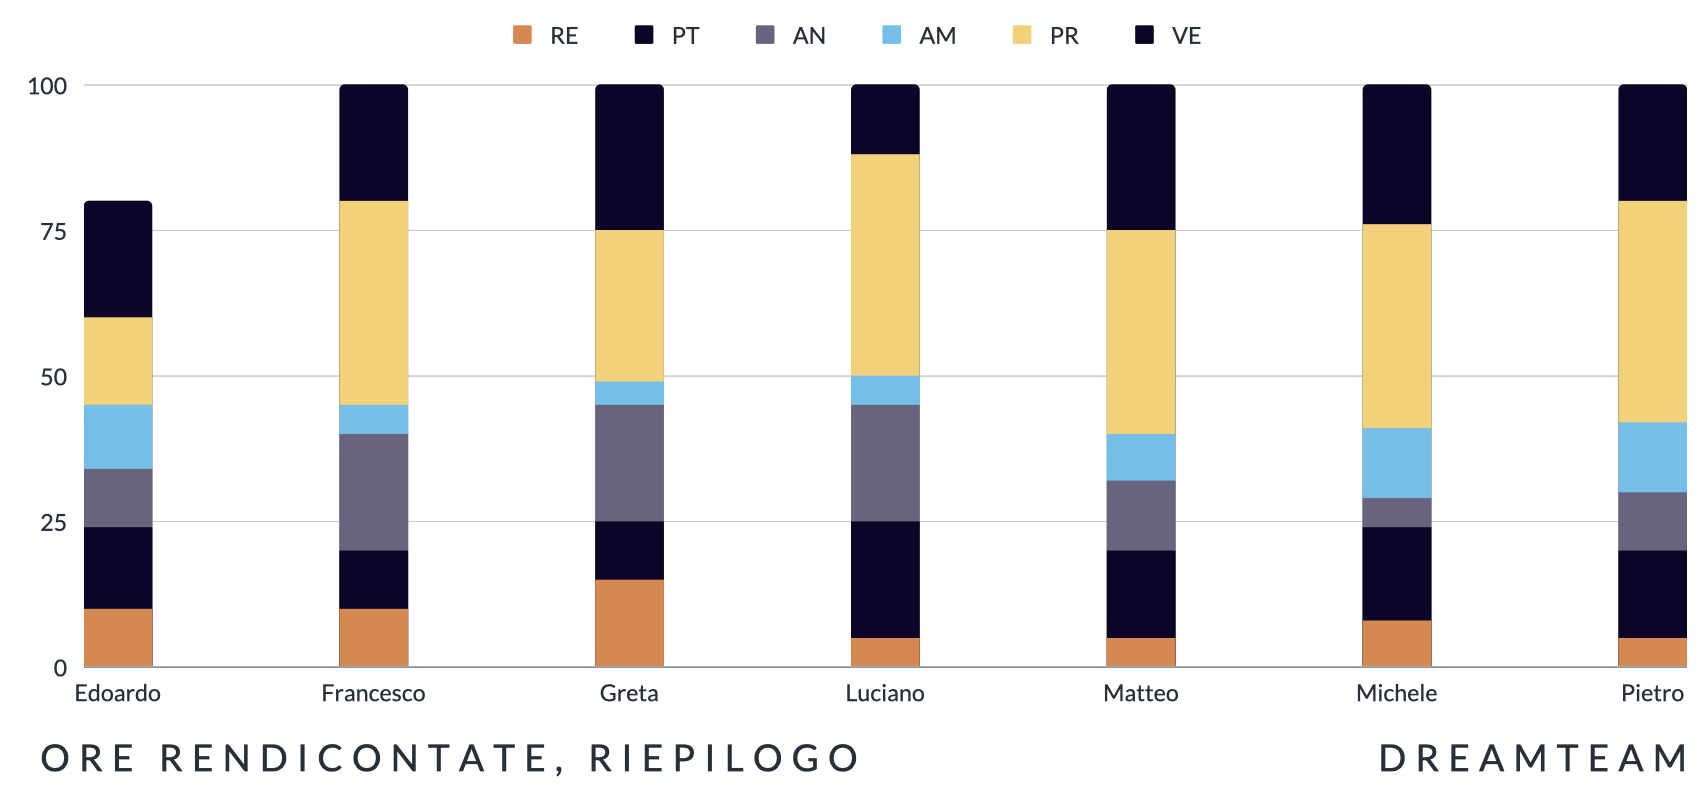
\includegraphics[scale=0.50]{Sezioni/SezioniPreventivo/grafici/Riepilogo_ore_rendicontate.png}
\caption{Istogramma della ripartizione delle ore rendicontate}
\end{figure}

\subsubsection{Prospetto economico}
La seguente tabella rappresenta le ore totali dedicate ad ogni ruolo e il costo in euro:

\begin{table}[H]
\begin{center}
\rowcolors{2}{gray!25}{white}
\renewcommand{\arraystretch}{1.5}
\begin{tabular}{ m{0.3\textwidth}<{\centering}  m{0.2\textwidth}<{\centering} m{0.2\textwidth}<{\centering}}
	\rowcolor{darkblue}
	\textcolor{white}{\textbf{Ruolo}}&\textcolor{white}{\textbf{Totale ore}}&\textcolor{white}{\textbf{Costo totale (\euro)}}\\ 

	Responsabile & 58 & 1740 \\	
	
	Progettista & 100 & 2500 \\
	
	Analista & 97 & 2425 \\

	Amministratore & 57 & 1140 \\
	
	Programmatore & 222 & 3330 \\
	
	Verificatore & 146 & 2190 \\
	
	\textbf{Totale} & 680 & 13325 \\
	
\end{tabular}
\caption{Prospetto dei costi totali delle ore rendicontate}
\end{center}
\end{table}

La tabella può essere rappresentata anche in forma visiva dal seguente aerogramma:
\begin{figure}[H]
\centering
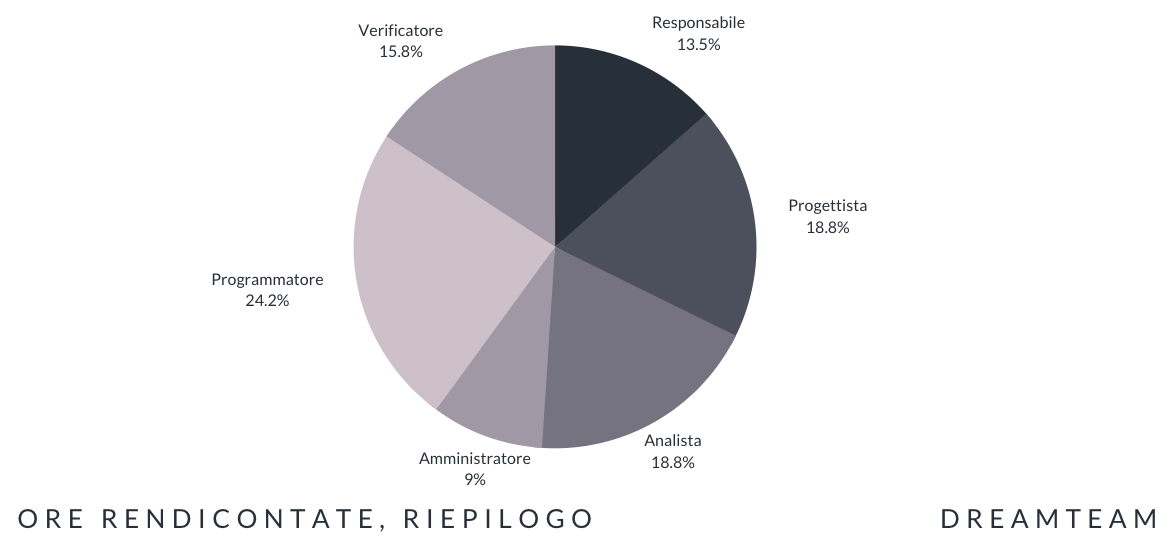
\includegraphics[scale=0.50]{Sezioni/SezioniPreventivo/grafici/Riepilogo_ore_rendicontate_costi.png}
\caption{Grafico a torta della ripartizione per ruolo delle ore rendicontate}
\end{figure}

\subsubsection{Conclusioni}
Il costo totale del progetto considerando solamente le ore rendicontate è: 13.325,00\euro.